\chapter{Introducción}

\section{Motivación}

Desde que era pequeño me ha llamado la atención el concepto enseñanza. El aprender...

compartir conocimientos
enseñar lo que se sabe




\blindtext

\section{Definición del problema}

\blindtext

Este proyecto intentará resolver los siguientes problemas:

\begin{itemize}
  \item Evitar la tediosa tarea de la corrección de ejercicios.
  \item Motivar la enseñanza y apredizaje de la programación a través de ejemplos.
  \item Ver como un sistema de control de versiones es una herramienta básica que debería enseñarse a la vez que se enseña programación.
  \item Mejorar la calidad de vida tanto de profesores como de estudiantes
\end{itemize}

\blindtext

\section{Estructura del proyecto}


\bigskip
Antes de pasar a detalles más técnicos, me gustaría detallar el contenido de este proyecto:

\begin{itemize}
  \item En el \textit{capítulo 1} (\textbf{Introducción}) se encuentra un texto descriptivo del proyecto, así como una breve introducción a las tecnologías que se utilizarán.
  \item El \textit{capítulo 2} (\textbf{Objetivos}) detalla de forma algo más concreta los objetivos determinados que se quieren cumplir con este proyecto.
  \item En el \textit{capítulo 3} (\textbf{Metodología}) está la planificación y desarrollo de cada uno de los apartados del proyecto.
  \item En el \textit{capítulo 4} (\textbf{Resultados})se detallan todos los resultados obtenidos.
  \item En el \textit{capítulo 5} (\textbf{Conclusiones}) se pueden encontrar las conclusiones finales  así como las recomendaciones para futuros trabajos.

\end{itemize}

\bigskip
Para finalizar se incluye un anexo con el código fuente desarrollado y liberado bajo una licencia libre.


% %
% % Ejemplos de codigo LaTeX para uso futuro
% %

% \begin{figure}[h!]
% \centering
% 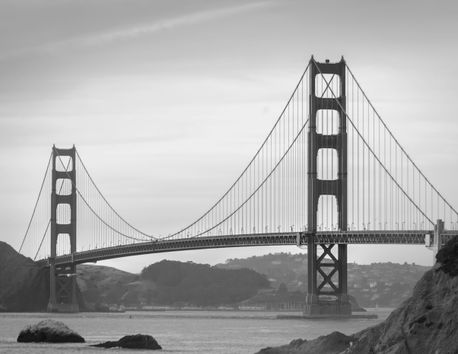
\includegraphics{../screenshots/sample1}
% \caption{Sample Image 1}
% \label{fig:sample1}
% \end{figure}

% Esto es un texto con una nota\footnote{Ejemplo de nota al pie} al pie.

% Y esto es una ``Frase de alguien''\cite{stevekrug}.

% \begin{itemize}
%   \item \textbf{1.} Texto de ejemplo
%   \item \textbf{2.} Texto de ejemplo
%   \item \textbf{3.} Texto de ejemplo
%   \item \textbf{4.} Texto de ejemplo

% \end{itemize}

% \begin{enumerate}
% 	\item Ejemplo 1.
% 	\item Ejemplo 2.
% \end{enumerate}

% \begin{lstlisting}[language=html]
% <!DOCTYPE html>
% <html lang="es-ES">
%   <head>
%     <meta charset="utf-8">
%     <title>Ejemplo de 2 párrafos</title>
%   </head>
%   <body>
%     <p>Esto es un párrafo.</p>
%     <p>Esto es otro párrafo.</p>
%   </body>
% </html>
% \end{lstlisting}

% Puedes verlo en \cite{Patricio2011}. Te recomiendo leer \cite{Patricio2011, Zacarias2009, Alfonso2010b, Alfonso2010a}.
